\section{Reihen}
\todo{% TODO: \usepackage{graphicx} required
	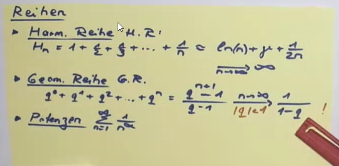
\includegraphics{Images/screenshot001}\\
}

\subsection{Reihen \bronstein{1077}}
oder \bronstein{157} von Buch.
\begin{align*}
	\sum_{k=1}^n k   &= \frac{n(n+1)}{2} &
	\sum_{k=1}^n k^2 &= \frac{n(n+1)(2n+1)}{6} \\
	\sum_{k=1}^n k^3 &= \frac{n^2(n+1)^2}{4} &
	\sum_{k=0}^{n-1} ar^k &= a\left(\frac{1-r^n}{1-r}\right) (r \neq 1)
\end{align*}


\subsection{Konvergenz/Divergenz}
\subsubsection{Raffsumme}
Summe von benachbarten Differenzen. Nur wenn letzter Summand $a_{n+1} \rightarrow 0$, dann konvergiert die Reihe.
Falls $\alpha = \lim_{n \rightarrow \infty} \neq 0$, dann Divergenz. $\alpha=0$ funktioniert nicht!

\subsubsection{Leibniz-Reihe}
Konvergenz zeichnet sich durch folgende Eigenschaften aus:
\begin{enumerate}[nosep]
	\item Vorzeichenwechsel
	\item Letzter Summand $\rightarrow 0$
	\item $\left|a_n\right|$ monoton fallend
\end{enumerate}

\subsubsection{Cauchy-Wurzelkriterium}\label{W-Kriterium}
\[\alpha = \lim\limits_{n \rightarrow \infty}{\sqrt[n]{\left|a_n\right|}}\qquad
\left\lbrace
\begin{array}{r@{}l}
	\alpha < 1 &: \text{dann} \sum a_n \text{Konvergenz} \\
	\alpha > 1 &: \text{dann} \sum a_n \text{Divergenz} \\
	\alpha = 1 &: \text{Keine Aussage} \\
\end{array}\right. \]
Falls keine Aussage getroffen werden kann, siehe auch Leibniz, Maj./Min. oder Quotientenkrit.
\\ \\
\noindent Hinweis:
\todo{limit superium, Woche 9}

\subsubsection{D'Alembert Quotientenkriterium}
\[\alpha = \lim\limits_{n \rightarrow \infty}{\frac{a_{n+1}}{a_n}}\]
Siehe \verweiseref{W-Kriterium}, auch für Hinweis.

\subsubsection{Integralkriterium}
Wenn das Integral konvergiert, dann auch die Reihe:
\[\int_{1}^{\infty}f(x)dx \quad\leq\quad \sum_{n=1}^{\infty}f(n)\]
Gilt nur wenn $f(x) \geq 0$ und $f$ fallend!

\subsubsection{Bedingt/Unbedingte Konvergenz}
\textbf{Bedingte Konvergenz}, durch Umordnen der Summanden können neue Summen enstehen, sogar Divergenz. Damit kann jede Zahl in $\mathbb{R}$ erreicht werden.\\
\textbf{Unbedingte Konvergenz} ändert die Summe nicht bei einer Umordung, kann geprüft werden mit der \textbf{Absoluten Konvergenz}:
\[\sum\left|a_n\right| < \infty\]

\subsubsection{Reihenentwicklung}
Weitere Referenzen in \bronstein{21.3}
\[\sum_{n = 0}^{\infty}1x^n = \frac{1}{1-x}\]
\todo{Fr. 20.4.21}

\subsection{Fehlerabschätzung}
\todo{Vorlesung - Reihe:$\left|s - s_n\right| \geq \left|a_{n+1}\right|$}

\subsection{Konvergenzradius}
\todo{\[\left|x - x_0\right| < \frac{1}{\lim\limits_{n \rightarrow \infty}\sqrt[n]{\left|a_n\right|}}\]}

\subsubsection{Konvergenzgeschwindigkeit}
\todo{Woche 10}

\subsubsection{Ableitung/Integrieren}
Ableitung:\[\sum_{n=i}^{\infty}n(n-1)\dots(n-i+1)a_nx^{n-i}=f^{(i)}(x)\]
Integration: \[\sum_{n=0}^{\infty}a_n\frac{x^{n+1}}{n+1}=\int f(x)dx+C\]
Hinweis: Für $C$, Konv.Radius-Zentrum $x_0$ einsetzen.
\todo{DI 4.5.21}